% Options for packages loaded elsewhere
\PassOptionsToPackage{unicode}{hyperref}
\PassOptionsToPackage{hyphens}{url}
%
\documentclass[
  english,
  man]{apa6}
\usepackage{lmodern}
\usepackage{amssymb,amsmath}
\usepackage{ifxetex,ifluatex}
\ifnum 0\ifxetex 1\fi\ifluatex 1\fi=0 % if pdftex
  \usepackage[T1]{fontenc}
  \usepackage[utf8]{inputenc}
  \usepackage{textcomp} % provide euro and other symbols
\else % if luatex or xetex
  \usepackage{unicode-math}
  \defaultfontfeatures{Scale=MatchLowercase}
  \defaultfontfeatures[\rmfamily]{Ligatures=TeX,Scale=1}
\fi
% Use upquote if available, for straight quotes in verbatim environments
\IfFileExists{upquote.sty}{\usepackage{upquote}}{}
\IfFileExists{microtype.sty}{% use microtype if available
  \usepackage[]{microtype}
  \UseMicrotypeSet[protrusion]{basicmath} % disable protrusion for tt fonts
}{}
\makeatletter
\@ifundefined{KOMAClassName}{% if non-KOMA class
  \IfFileExists{parskip.sty}{%
    \usepackage{parskip}
  }{% else
    \setlength{\parindent}{0pt}
    \setlength{\parskip}{6pt plus 2pt minus 1pt}}
}{% if KOMA class
  \KOMAoptions{parskip=half}}
\makeatother
\usepackage{xcolor}
\IfFileExists{xurl.sty}{\usepackage{xurl}}{} % add URL line breaks if available
\IfFileExists{bookmark.sty}{\usepackage{bookmark}}{\usepackage{hyperref}}
\hypersetup{
  pdftitle={MSDS680 - Week 5 - ANN and SVM},
  pdfauthor={Benjamin Siebold},
  pdflang={en-EN},
  pdfkeywords={keywords},
  hidelinks,
  pdfcreator={LaTeX via pandoc}}
\urlstyle{same} % disable monospaced font for URLs
\usepackage{color}
\usepackage{fancyvrb}
\newcommand{\VerbBar}{|}
\newcommand{\VERB}{\Verb[commandchars=\\\{\}]}
\DefineVerbatimEnvironment{Highlighting}{Verbatim}{commandchars=\\\{\}}
% Add ',fontsize=\small' for more characters per line
\usepackage{framed}
\definecolor{shadecolor}{RGB}{248,248,248}
\newenvironment{Shaded}{\begin{snugshade}}{\end{snugshade}}
\newcommand{\AlertTok}[1]{\textcolor[rgb]{0.94,0.16,0.16}{#1}}
\newcommand{\AnnotationTok}[1]{\textcolor[rgb]{0.56,0.35,0.01}{\textbf{\textit{#1}}}}
\newcommand{\AttributeTok}[1]{\textcolor[rgb]{0.77,0.63,0.00}{#1}}
\newcommand{\BaseNTok}[1]{\textcolor[rgb]{0.00,0.00,0.81}{#1}}
\newcommand{\BuiltInTok}[1]{#1}
\newcommand{\CharTok}[1]{\textcolor[rgb]{0.31,0.60,0.02}{#1}}
\newcommand{\CommentTok}[1]{\textcolor[rgb]{0.56,0.35,0.01}{\textit{#1}}}
\newcommand{\CommentVarTok}[1]{\textcolor[rgb]{0.56,0.35,0.01}{\textbf{\textit{#1}}}}
\newcommand{\ConstantTok}[1]{\textcolor[rgb]{0.00,0.00,0.00}{#1}}
\newcommand{\ControlFlowTok}[1]{\textcolor[rgb]{0.13,0.29,0.53}{\textbf{#1}}}
\newcommand{\DataTypeTok}[1]{\textcolor[rgb]{0.13,0.29,0.53}{#1}}
\newcommand{\DecValTok}[1]{\textcolor[rgb]{0.00,0.00,0.81}{#1}}
\newcommand{\DocumentationTok}[1]{\textcolor[rgb]{0.56,0.35,0.01}{\textbf{\textit{#1}}}}
\newcommand{\ErrorTok}[1]{\textcolor[rgb]{0.64,0.00,0.00}{\textbf{#1}}}
\newcommand{\ExtensionTok}[1]{#1}
\newcommand{\FloatTok}[1]{\textcolor[rgb]{0.00,0.00,0.81}{#1}}
\newcommand{\FunctionTok}[1]{\textcolor[rgb]{0.00,0.00,0.00}{#1}}
\newcommand{\ImportTok}[1]{#1}
\newcommand{\InformationTok}[1]{\textcolor[rgb]{0.56,0.35,0.01}{\textbf{\textit{#1}}}}
\newcommand{\KeywordTok}[1]{\textcolor[rgb]{0.13,0.29,0.53}{\textbf{#1}}}
\newcommand{\NormalTok}[1]{#1}
\newcommand{\OperatorTok}[1]{\textcolor[rgb]{0.81,0.36,0.00}{\textbf{#1}}}
\newcommand{\OtherTok}[1]{\textcolor[rgb]{0.56,0.35,0.01}{#1}}
\newcommand{\PreprocessorTok}[1]{\textcolor[rgb]{0.56,0.35,0.01}{\textit{#1}}}
\newcommand{\RegionMarkerTok}[1]{#1}
\newcommand{\SpecialCharTok}[1]{\textcolor[rgb]{0.00,0.00,0.00}{#1}}
\newcommand{\SpecialStringTok}[1]{\textcolor[rgb]{0.31,0.60,0.02}{#1}}
\newcommand{\StringTok}[1]{\textcolor[rgb]{0.31,0.60,0.02}{#1}}
\newcommand{\VariableTok}[1]{\textcolor[rgb]{0.00,0.00,0.00}{#1}}
\newcommand{\VerbatimStringTok}[1]{\textcolor[rgb]{0.31,0.60,0.02}{#1}}
\newcommand{\WarningTok}[1]{\textcolor[rgb]{0.56,0.35,0.01}{\textbf{\textit{#1}}}}
\usepackage{graphicx,grffile}
\makeatletter
\def\maxwidth{\ifdim\Gin@nat@width>\linewidth\linewidth\else\Gin@nat@width\fi}
\def\maxheight{\ifdim\Gin@nat@height>\textheight\textheight\else\Gin@nat@height\fi}
\makeatother
% Scale images if necessary, so that they will not overflow the page
% margins by default, and it is still possible to overwrite the defaults
% using explicit options in \includegraphics[width, height, ...]{}
\setkeys{Gin}{width=\maxwidth,height=\maxheight,keepaspectratio}
% Set default figure placement to htbp
\makeatletter
\def\fps@figure{htbp}
\makeatother
\setlength{\emergencystretch}{3em} % prevent overfull lines
\providecommand{\tightlist}{%
  \setlength{\itemsep}{0pt}\setlength{\parskip}{0pt}}
\setcounter{secnumdepth}{-\maxdimen} % remove section numbering
% Make \paragraph and \subparagraph free-standing
\ifx\paragraph\undefined\else
  \let\oldparagraph\paragraph
  \renewcommand{\paragraph}[1]{\oldparagraph{#1}\mbox{}}
\fi
\ifx\subparagraph\undefined\else
  \let\oldsubparagraph\subparagraph
  \renewcommand{\subparagraph}[1]{\oldsubparagraph{#1}\mbox{}}
\fi
% Manuscript styling
\usepackage{upgreek}
\captionsetup{font=singlespacing,justification=justified}

% Table formatting
\usepackage{longtable}
\usepackage{lscape}
% \usepackage[counterclockwise]{rotating}   % Landscape page setup for large tables
\usepackage{multirow}		% Table styling
\usepackage{tabularx}		% Control Column width
\usepackage[flushleft]{threeparttable}	% Allows for three part tables with a specified notes section
\usepackage{threeparttablex}            % Lets threeparttable work with longtable

% Create new environments so endfloat can handle them
% \newenvironment{ltable}
%   {\begin{landscape}\begin{center}\begin{threeparttable}}
%   {\end{threeparttable}\end{center}\end{landscape}}
\newenvironment{lltable}{\begin{landscape}\begin{center}\begin{ThreePartTable}}{\end{ThreePartTable}\end{center}\end{landscape}}

% Enables adjusting longtable caption width to table width
% Solution found at http://golatex.de/longtable-mit-caption-so-breit-wie-die-tabelle-t15767.html
\makeatletter
\newcommand\LastLTentrywidth{1em}
\newlength\longtablewidth
\setlength{\longtablewidth}{1in}
\newcommand{\getlongtablewidth}{\begingroup \ifcsname LT@\roman{LT@tables}\endcsname \global\longtablewidth=0pt \renewcommand{\LT@entry}[2]{\global\advance\longtablewidth by ##2\relax\gdef\LastLTentrywidth{##2}}\@nameuse{LT@\roman{LT@tables}} \fi \endgroup}

% \setlength{\parindent}{0.5in}
% \setlength{\parskip}{0pt plus 0pt minus 0pt}

% \usepackage{etoolbox}
\makeatletter
\patchcmd{\HyOrg@maketitle}
  {\section{\normalfont\normalsize\abstractname}}
  {\section*{\normalfont\normalsize\abstractname}}
  {}{\typeout{Failed to patch abstract.}}
\patchcmd{\HyOrg@maketitle}
  {\section{\protect\normalfont{\@title}}}
  {\section*{\protect\normalfont{\@title}}}
  {}{\typeout{Failed to patch title.}}
\makeatother
\shorttitle{ANN and SVM}
\keywords{keywords\newline\indent Word count: X}
\DeclareDelayedFloatFlavor{ThreePartTable}{table}
\DeclareDelayedFloatFlavor{lltable}{table}
\DeclareDelayedFloatFlavor*{longtable}{table}
\makeatletter
\renewcommand{\efloat@iwrite}[1]{\immediate\expandafter\protected@write\csname efloat@post#1\endcsname{}}
\makeatother
\usepackage{csquotes}
\ifxetex
  % Load polyglossia as late as possible: uses bidi with RTL langages (e.g. Hebrew, Arabic)
  \usepackage{polyglossia}
  \setmainlanguage[]{english}
\else
  \usepackage[shorthands=off,main=english]{babel}
\fi

\title{MSDS680 - Week 5 - ANN and SVM}
\author{Benjamin Siebold\textsuperscript{}}
\date{}


\affiliation{\vspace{0.5cm}\textsuperscript{} Regis University}

\begin{document}
\maketitle

\hypertarget{introduction}{%
\section{Introduction}\label{introduction}}

In this project, both Support Vector Machines and Neural Networks will be explored using the Mushroom dataset from UCI to predict whether or not a mushroom is edible or poisonous. The mushroom dataset contains 8124 rows and 23 variables. This includes 22 features and one label (edible, poisionous). The muhsroom dataset does not include full descriptions of each feature, rather an abbreviation or indicator for every variable. These features are attributes of the mushroom, such as color, texture, smell, along with where it grows. To access the dataset and find the values for each column please refer to \url{http://archive.ics.uci.edu/ml/machine-learning-databases/mushroom/}.

\hypertarget{methodology}{%
\section{Methodology}\label{methodology}}

\hypertarget{set-up}{%
\subsection{Set up}\label{set-up}}

As is the first step in any analysis, the data needs to be loaded in, the necessary libraries and packages for exploration, cleaning, and model application need to be installed and loaded int the instance, the seed is set for repeateable results, and because there are not column names in the reading of the data in this instance column names will be applied to the dataset.

\begin{Shaded}
\begin{Highlighting}[]
\KeywordTok{library}\NormalTok{(data.table) }\CommentTok{#used to read in data}
\KeywordTok{library}\NormalTok{(DataExplorer)}\CommentTok{#used to inspect the data and get initial understanding}
\KeywordTok{library}\NormalTok{(e1071) }\CommentTok{#used for SVM model}
\KeywordTok{library}\NormalTok{(caret) }\CommentTok{#used for model analysis}
\KeywordTok{library}\NormalTok{(class) }\CommentTok{#used for converting data types}
\KeywordTok{library}\NormalTok{(dbplyr) }\CommentTok{#used for removing/adding columns}
\KeywordTok{library}\NormalTok{(neuralnet) }\CommentTok{#used for neural net model}

\KeywordTok{set.seed}\NormalTok{(}\DecValTok{476}\NormalTok{)}

\NormalTok{mushroom_data <-}\StringTok{ }\KeywordTok{read.table}\NormalTok{(}
  \StringTok{'http://archive.ics.uci.edu/ml/machine-learning-databases/mushroom/agaricus-lepiota.data'}\NormalTok{, }
  \DataTypeTok{stringsAsFactors =}\NormalTok{ T, }\DataTypeTok{header =}\NormalTok{ F, }\DataTypeTok{sep =} \StringTok{','}\NormalTok{)}

\NormalTok{col_names <-}\StringTok{ }\KeywordTok{c}\NormalTok{(}\StringTok{'class'}\NormalTok{, }\StringTok{'cap.shape'}\NormalTok{, }\StringTok{'cap.surface'}\NormalTok{, }\StringTok{'cap.clr'}\NormalTok{, }\StringTok{'bruises'}\NormalTok{, }\StringTok{'odor'}\NormalTok{,}
               \StringTok{'gill.attach'}\NormalTok{, }\StringTok{'gill.spacing'}\NormalTok{, }\StringTok{'gill.sz'}\NormalTok{, }\StringTok{'gill.clr'}\NormalTok{,}
               \StringTok{'stalk.shape'}\NormalTok{, }\StringTok{'stalk.root'}\NormalTok{, }\StringTok{'stalk.sar'}\NormalTok{, }\StringTok{'stalk.sbr'}\NormalTok{,}
               \StringTok{'stalk.clr.abv.rng'}\NormalTok{, }\StringTok{'stalk.clr.bel.rng'}\NormalTok{, }\StringTok{'veil.type'}\NormalTok{, }\StringTok{'veil.clr'}\NormalTok{,}
               \StringTok{'ring.num'}\NormalTok{, }\StringTok{'ring.type'}\NormalTok{, }\StringTok{'spore.prnt.clr'}\NormalTok{, }\StringTok{'pop'}\NormalTok{, }\StringTok{'habitat'}\NormalTok{)}

\KeywordTok{names}\NormalTok{(mushroom_data) <-}\StringTok{ }\NormalTok{col_names}
\end{Highlighting}
\end{Shaded}

\hypertarget{data-exploration}{%
\subsection{Data Exploration}\label{data-exploration}}

With the data loaded, exploration of what exists in the data can begin.

\begin{Shaded}
\begin{Highlighting}[]
\CommentTok{# initial data inspectio}
\KeywordTok{summary}\NormalTok{(mushroom_data) }\CommentTok{# provides initial idea of what data looks like}
\end{Highlighting}
\end{Shaded}

\begin{verbatim}
##  class    cap.shape cap.surface    cap.clr     bruises       odor     
##  e:4208   b: 452    f:2320      n      :2284   f:4748   n      :3528  
##  p:3916   c:   4    g:   4      g      :1840   t:3376   f      :2160  
##           f:3152    s:2556      e      :1500            s      : 576  
##           k: 828    y:3244      y      :1072            y      : 576  
##           s:  32                w      :1040            a      : 400  
##           x:3656                b      : 168            l      : 400  
##                                 (Other): 220            (Other): 484  
##  gill.attach gill.spacing gill.sz     gill.clr    stalk.shape stalk.root
##  a: 210      c:6812       b:5612   b      :1728   e:3516      ?:2480    
##  f:7914      w:1312       n:2512   p      :1492   t:4608      b:3776    
##                                    w      :1202               c: 556    
##                                    n      :1048               e:1120    
##                                    g      : 752               r: 192    
##                                    h      : 732                         
##                                    (Other):1170                         
##  stalk.sar stalk.sbr stalk.clr.abv.rng stalk.clr.bel.rng veil.type veil.clr
##  f: 552    f: 600    w      :4464      w      :4384      p:8124    n:  96  
##  k:2372    k:2304    p      :1872      p      :1872                o:  96  
##  s:5176    s:4936    g      : 576      g      : 576                w:7924  
##  y:  24    y: 284    n      : 448      n      : 512                y:   8  
##                      b      : 432      b      : 432                        
##                      o      : 192      o      : 192                        
##                      (Other): 140      (Other): 156                        
##  ring.num ring.type spore.prnt.clr pop      habitat 
##  n:  36   e:2776    w      :2388   a: 384   d:3148  
##  o:7488   f:  48    n      :1968   c: 340   g:2148  
##  t: 600   l:1296    k      :1872   n: 400   l: 832  
##           n:  36    h      :1632   s:1248   m: 292  
##           p:3968    r      :  72   v:4040   p:1144  
##                     b      :  48   y:1712   u: 368  
##                     (Other): 144            w: 192
\end{verbatim}

\begin{Shaded}
\begin{Highlighting}[]
\KeywordTok{plot_intro}\NormalTok{(mushroom_data)}
\end{Highlighting}
\end{Shaded}

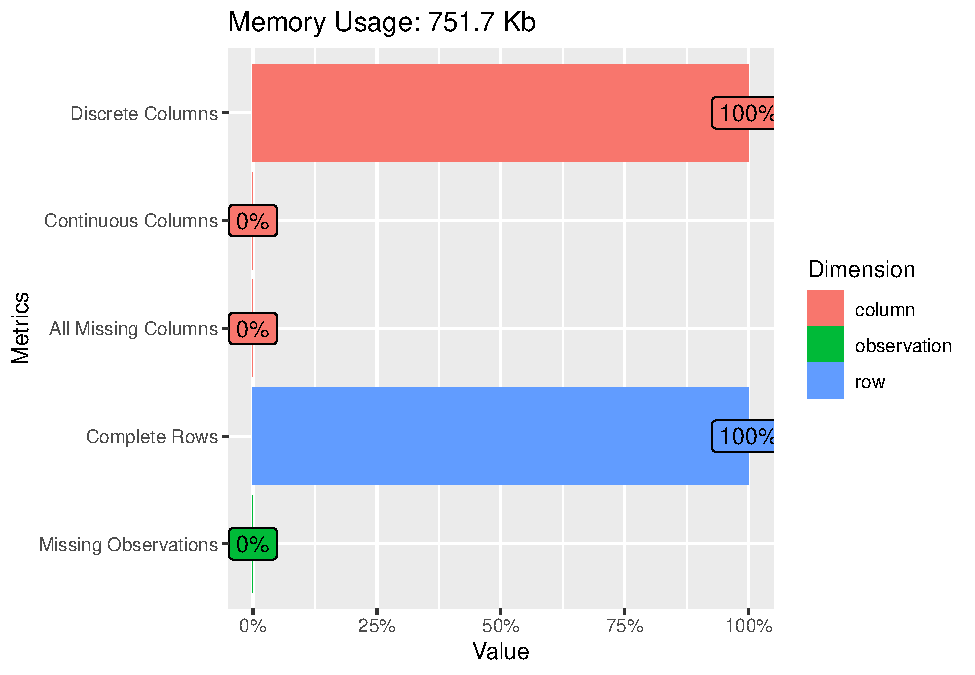
\includegraphics{MSDS680-Week-5-SVM-and-ANNRmd_files/figure-latex/data exploration-1.pdf}

\begin{Shaded}
\begin{Highlighting}[]
\KeywordTok{plot_missing}\NormalTok{(mushroom_data)}
\end{Highlighting}
\end{Shaded}

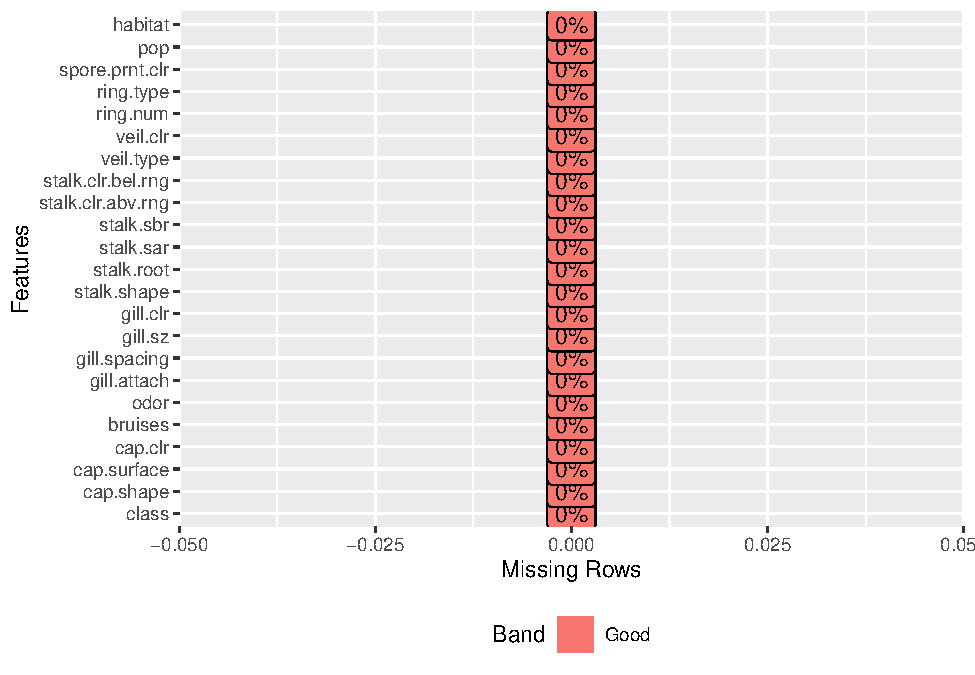
\includegraphics{MSDS680-Week-5-SVM-and-ANNRmd_files/figure-latex/data exploration-2.pdf}

\begin{Shaded}
\begin{Highlighting}[]
\KeywordTok{plot_correlation}\NormalTok{(mushroom_data)}
\end{Highlighting}
\end{Shaded}

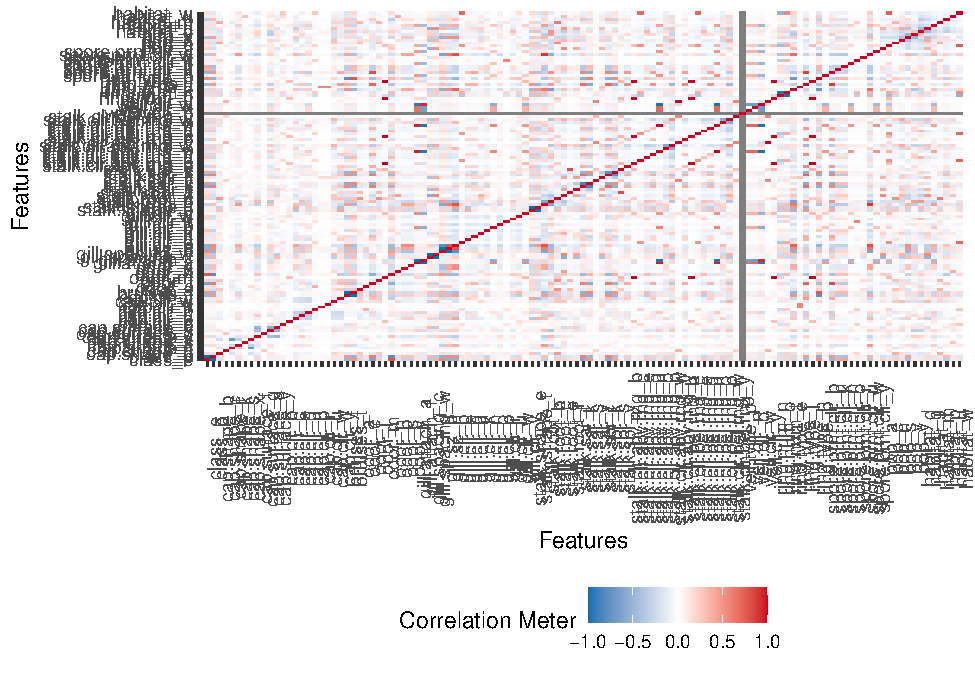
\includegraphics{MSDS680-Week-5-SVM-and-ANNRmd_files/figure-latex/data exploration-3.pdf}

\begin{Shaded}
\begin{Highlighting}[]
\KeywordTok{str}\NormalTok{(mushroom_data)}
\end{Highlighting}
\end{Shaded}

\begin{verbatim}
## 'data.frame':    8124 obs. of  23 variables:
##  $ class            : Factor w/ 2 levels "e","p": 2 1 1 2 1 1 1 1 2 1 ...
##  $ cap.shape        : Factor w/ 6 levels "b","c","f","k",..: 6 6 1 6 6 6 1 1 6 1 ...
##  $ cap.surface      : Factor w/ 4 levels "f","g","s","y": 3 3 3 4 3 4 3 4 4 3 ...
##  $ cap.clr          : Factor w/ 10 levels "b","c","e","g",..: 5 10 9 9 4 10 9 9 9 10 ...
##  $ bruises          : Factor w/ 2 levels "f","t": 2 2 2 2 1 2 2 2 2 2 ...
##  $ odor             : Factor w/ 9 levels "a","c","f","l",..: 7 1 4 7 6 1 1 4 7 1 ...
##  $ gill.attach      : Factor w/ 2 levels "a","f": 2 2 2 2 2 2 2 2 2 2 ...
##  $ gill.spacing     : Factor w/ 2 levels "c","w": 1 1 1 1 2 1 1 1 1 1 ...
##  $ gill.sz          : Factor w/ 2 levels "b","n": 2 1 1 2 1 1 1 1 2 1 ...
##  $ gill.clr         : Factor w/ 12 levels "b","e","g","h",..: 5 5 6 6 5 6 3 6 8 3 ...
##  $ stalk.shape      : Factor w/ 2 levels "e","t": 1 1 1 1 2 1 1 1 1 1 ...
##  $ stalk.root       : Factor w/ 5 levels "?","b","c","e",..: 4 3 3 4 4 3 3 3 4 3 ...
##  $ stalk.sar        : Factor w/ 4 levels "f","k","s","y": 3 3 3 3 3 3 3 3 3 3 ...
##  $ stalk.sbr        : Factor w/ 4 levels "f","k","s","y": 3 3 3 3 3 3 3 3 3 3 ...
##  $ stalk.clr.abv.rng: Factor w/ 9 levels "b","c","e","g",..: 8 8 8 8 8 8 8 8 8 8 ...
##  $ stalk.clr.bel.rng: Factor w/ 9 levels "b","c","e","g",..: 8 8 8 8 8 8 8 8 8 8 ...
##  $ veil.type        : Factor w/ 1 level "p": 1 1 1 1 1 1 1 1 1 1 ...
##  $ veil.clr         : Factor w/ 4 levels "n","o","w","y": 3 3 3 3 3 3 3 3 3 3 ...
##  $ ring.num         : Factor w/ 3 levels "n","o","t": 2 2 2 2 2 2 2 2 2 2 ...
##  $ ring.type        : Factor w/ 5 levels "e","f","l","n",..: 5 5 5 5 1 5 5 5 5 5 ...
##  $ spore.prnt.clr   : Factor w/ 9 levels "b","h","k","n",..: 3 4 4 3 4 3 3 4 3 3 ...
##  $ pop              : Factor w/ 6 levels "a","c","n","s",..: 4 3 3 4 1 3 3 4 5 4 ...
##  $ habitat          : Factor w/ 7 levels "d","g","l","m",..: 6 2 4 6 2 2 4 4 2 4 ...
\end{verbatim}

Above a few visuals show inspecting the data is quite difficult in its current state. To allow for easier inspection of the data, it has been converted to factors. A few aspects of the data are interesting. For example vei.type only has one value and thus can be removed. Additionally stalk.root has almost one third of the data being \enquote{?}. To fall in line with the rest of the column, the question marks will be converted to \enquote{u} for unknown.

\begin{Shaded}
\begin{Highlighting}[]
\NormalTok{shroom_dat <-}\StringTok{ }\KeywordTok{subset}\NormalTok{(mushroom_data, }\DataTypeTok{select =} \OperatorTok{-}\KeywordTok{c}\NormalTok{(}\StringTok{`}\DataTypeTok{veil.type}\StringTok{`}\NormalTok{))}
\KeywordTok{levels}\NormalTok{(shroom_dat}\OperatorTok{$}\StringTok{`}\DataTypeTok{stalk.root}\StringTok{`}\NormalTok{)[}\KeywordTok{levels}\NormalTok{(shroom_dat}\OperatorTok{$}\StringTok{`}\DataTypeTok{stalk.root}\StringTok{`}\NormalTok{)}\OperatorTok{==}\StringTok{"?"}\NormalTok{] <-}\StringTok{ "u"} \CommentTok{#converts missing data to "unknown"}

\NormalTok{shroom_dat}\OperatorTok{$}\NormalTok{class <-}\StringTok{ }\KeywordTok{as.factor}\NormalTok{(shroom_dat}\OperatorTok{$}\NormalTok{class)}
\KeywordTok{str}\NormalTok{(shroom_dat)}
\end{Highlighting}
\end{Shaded}

\begin{verbatim}
## 'data.frame':    8124 obs. of  22 variables:
##  $ class            : Factor w/ 2 levels "e","p": 2 1 1 2 1 1 1 1 2 1 ...
##  $ cap.shape        : Factor w/ 6 levels "b","c","f","k",..: 6 6 1 6 6 6 1 1 6 1 ...
##  $ cap.surface      : Factor w/ 4 levels "f","g","s","y": 3 3 3 4 3 4 3 4 4 3 ...
##  $ cap.clr          : Factor w/ 10 levels "b","c","e","g",..: 5 10 9 9 4 10 9 9 9 10 ...
##  $ bruises          : Factor w/ 2 levels "f","t": 2 2 2 2 1 2 2 2 2 2 ...
##  $ odor             : Factor w/ 9 levels "a","c","f","l",..: 7 1 4 7 6 1 1 4 7 1 ...
##  $ gill.attach      : Factor w/ 2 levels "a","f": 2 2 2 2 2 2 2 2 2 2 ...
##  $ gill.spacing     : Factor w/ 2 levels "c","w": 1 1 1 1 2 1 1 1 1 1 ...
##  $ gill.sz          : Factor w/ 2 levels "b","n": 2 1 1 2 1 1 1 1 2 1 ...
##  $ gill.clr         : Factor w/ 12 levels "b","e","g","h",..: 5 5 6 6 5 6 3 6 8 3 ...
##  $ stalk.shape      : Factor w/ 2 levels "e","t": 1 1 1 1 2 1 1 1 1 1 ...
##  $ stalk.root       : Factor w/ 5 levels "u","b","c","e",..: 4 3 3 4 4 3 3 3 4 3 ...
##  $ stalk.sar        : Factor w/ 4 levels "f","k","s","y": 3 3 3 3 3 3 3 3 3 3 ...
##  $ stalk.sbr        : Factor w/ 4 levels "f","k","s","y": 3 3 3 3 3 3 3 3 3 3 ...
##  $ stalk.clr.abv.rng: Factor w/ 9 levels "b","c","e","g",..: 8 8 8 8 8 8 8 8 8 8 ...
##  $ stalk.clr.bel.rng: Factor w/ 9 levels "b","c","e","g",..: 8 8 8 8 8 8 8 8 8 8 ...
##  $ veil.clr         : Factor w/ 4 levels "n","o","w","y": 3 3 3 3 3 3 3 3 3 3 ...
##  $ ring.num         : Factor w/ 3 levels "n","o","t": 2 2 2 2 2 2 2 2 2 2 ...
##  $ ring.type        : Factor w/ 5 levels "e","f","l","n",..: 5 5 5 5 1 5 5 5 5 5 ...
##  $ spore.prnt.clr   : Factor w/ 9 levels "b","h","k","n",..: 3 4 4 3 4 3 3 4 3 3 ...
##  $ pop              : Factor w/ 6 levels "a","c","n","s",..: 4 3 3 4 1 3 3 4 5 4 ...
##  $ habitat          : Factor w/ 7 levels "d","g","l","m",..: 6 2 4 6 2 2 4 4 2 4 ...
\end{verbatim}

\hypertarget{svm-model}{%
\subsection{SVM Model}\label{svm-model}}

The data is ready to be split and models are ready to be applied. The first model that will be used is the Support Vector Machine, which creates planes based off features to classify the data to either \enquote{edible} or \enquote{poisonous}. For curiosity sake, all four types of the SVM models will be applied to compare how they impact results. SVM models traditionally require numeric data in order for them to function; however, the library e1071 interprets the data as numeric based off classifying each label or category as a number.

\begin{Shaded}
\begin{Highlighting}[]
\NormalTok{idx <-}\StringTok{ }\KeywordTok{createDataPartition}\NormalTok{(shroom_dat}\OperatorTok{$}\NormalTok{class, }\DataTypeTok{p=}\FloatTok{0.7}\NormalTok{, }\DataTypeTok{list=}\OtherTok{FALSE}\NormalTok{) }\CommentTok{#creates index to split data}

\NormalTok{shroom_train <-}\StringTok{ }\NormalTok{shroom_dat[idx,]}
\NormalTok{shroom_test <-}\StringTok{ }\NormalTok{shroom_dat[}\OperatorTok{-}\NormalTok{idx,] }

\NormalTok{svm_linear <-}\StringTok{ }\KeywordTok{svm}\NormalTok{(class}\OperatorTok{~}\NormalTok{., }\DataTypeTok{data=}\NormalTok{shroom_train, }\DataTypeTok{type=}\StringTok{'C-classification'}\NormalTok{, }\DataTypeTok{kernel=}\StringTok{'linear'}\NormalTok{) }\CommentTok{# applies svm with a linear fit}
\NormalTok{shroom_lin_pred <-}\StringTok{ }\KeywordTok{predict}\NormalTok{(svm_linear, shroom_test)}
\NormalTok{svm_radial <-}\StringTok{ }\KeywordTok{svm}\NormalTok{(class}\OperatorTok{~}\NormalTok{., }\DataTypeTok{data=}\NormalTok{shroom_train, }\DataTypeTok{type=}\StringTok{'C-classification'}\NormalTok{, }\DataTypeTok{kernel=}\StringTok{'radial'}\NormalTok{) }\CommentTok{# applies svm with a radial fit}
\NormalTok{shroom_rad_pred <-}\StringTok{ }\KeywordTok{predict}\NormalTok{(svm_radial, shroom_test)}
\NormalTok{svm_poly <-}\StringTok{ }\KeywordTok{svm}\NormalTok{(class}\OperatorTok{~}\NormalTok{., }\DataTypeTok{data=}\NormalTok{shroom_train, }\DataTypeTok{type=}\StringTok{'C-classification'}\NormalTok{, }\DataTypeTok{kernel=}\StringTok{'polynomial'}\NormalTok{) }\CommentTok{# applies svm with a polynomial fit}
\NormalTok{shroom_poly_pred <-}\StringTok{ }\KeywordTok{predict}\NormalTok{(svm_poly, shroom_test)}
\NormalTok{svm_sigmoid <-}\StringTok{ }\KeywordTok{svm}\NormalTok{(class}\OperatorTok{~}\NormalTok{., }\DataTypeTok{data=}\NormalTok{shroom_train, }\DataTypeTok{type=}\StringTok{'C-classification'}\NormalTok{, }\DataTypeTok{kernel=}\StringTok{'sigmoid'}\NormalTok{) }\CommentTok{# applies svm with a sigmoid fit}
\NormalTok{shroom_sig_pred <-}\StringTok{ }\KeywordTok{predict}\NormalTok{(svm_sigmoid, shroom_test)}

\KeywordTok{confusionMatrix}\NormalTok{(shroom_lin_pred, shroom_test}\OperatorTok{$}\NormalTok{class)}\OperatorTok{$}\NormalTok{table }
\end{Highlighting}
\end{Shaded}

\begin{verbatim}
##           Reference
## Prediction    e    p
##          e 1262    0
##          p    0 1174
\end{verbatim}

\begin{Shaded}
\begin{Highlighting}[]
\KeywordTok{confusionMatrix}\NormalTok{(shroom_rad_pred, shroom_test}\OperatorTok{$}\NormalTok{class)}\OperatorTok{$}\NormalTok{table}
\end{Highlighting}
\end{Shaded}

\begin{verbatim}
##           Reference
## Prediction    e    p
##          e 1262    3
##          p    0 1171
\end{verbatim}

\begin{Shaded}
\begin{Highlighting}[]
\KeywordTok{confusionMatrix}\NormalTok{(shroom_poly_pred, shroom_test}\OperatorTok{$}\NormalTok{class)}\OperatorTok{$}\NormalTok{table}
\end{Highlighting}
\end{Shaded}

\begin{verbatim}
##           Reference
## Prediction    e    p
##          e 1248  148
##          p   14 1026
\end{verbatim}

\begin{Shaded}
\begin{Highlighting}[]
\KeywordTok{confusionMatrix}\NormalTok{(shroom_sig_pred, shroom_test}\OperatorTok{$}\NormalTok{class)}\OperatorTok{$}\NormalTok{table}
\end{Highlighting}
\end{Shaded}

\begin{verbatim}
##           Reference
## Prediction    e    p
##          e 1262   30
##          p    0 1144
\end{verbatim}

From applying the SVM models above, it can be seen the linear model and the radial model both perform similarly, while the polynomial and sigmoid models struggle. Due to the complexity of the data, even though the radial model is slightly less accurate it is recommended to apply this model to future, unknown data.

\hypertarget{neural-network}{%
\subsection{Neural Network}\label{neural-network}}

Another model that could work well for the analysis of the mushroom dataset are neural networks. These models operate by mimicking neural networks in the brain of humans, but at a much less complicated level. One caveat of neural networks is there is an absolute requirement that the data is numerical. Because of this, two different approaches will be used: One that replaces the data with dummy variables, and Two one that converts the categorical data to numeric.

\hypertarget{dummy-variable-test}{%
\subsubsection{Dummy Variable test}\label{dummy-variable-test}}

The first neural network to be built converts the data into many columns of booleans if a label is met. For example if there is a column with three categories, it will be split into three columns. Once this is done, the data is split into training and test data. Additionally, the training columns need to be assigned for the network formula to be built.

\begin{Shaded}
\begin{Highlighting}[]
\NormalTok{shroom_features <-}\StringTok{ }\KeywordTok{subset}\NormalTok{(shroom_dat, }\DataTypeTok{select =} \OperatorTok{-}\NormalTok{class) }\CommentTok{#removing class to dummy variable for ANN}
\NormalTok{shroom_Dummy <-}\StringTok{ }\KeywordTok{dummyVars}\NormalTok{(}\OperatorTok{~}\NormalTok{., }\DataTypeTok{data=}\NormalTok{shroom_features) }\CommentTok{#applies levels to variables for splitting factors}
\NormalTok{shroom_Dummy <-}\StringTok{ }\KeywordTok{data.frame}\NormalTok{(}\KeywordTok{predict}\NormalTok{(shroom_Dummy, shroom_features)) }\CommentTok{#transforms data into boolean columns for each level of factors}
\NormalTok{shroom_Dummy}\OperatorTok{$}\NormalTok{class <-}\StringTok{ }\NormalTok{shroom_dat}\OperatorTok{$}\NormalTok{class}
\KeywordTok{ncol}\NormalTok{(shroom_Dummy)}
\end{Highlighting}
\end{Shaded}

\begin{verbatim}
## [1] 117
\end{verbatim}

\begin{Shaded}
\begin{Highlighting}[]
\NormalTok{idx <-}\StringTok{ }\KeywordTok{createDataPartition}\NormalTok{(shroom_Dummy}\OperatorTok{$}\NormalTok{class, }\DataTypeTok{p=}\FloatTok{0.7}\NormalTok{, }\DataTypeTok{list=}\OtherTok{FALSE}\NormalTok{) }\CommentTok{#creates index to split data}
\NormalTok{ann_shroom_train <-}\StringTok{ }\NormalTok{shroom_Dummy[idx,]}
\NormalTok{ann_shroom_test <-}\StringTok{ }\NormalTok{shroom_Dummy[}\OperatorTok{-}\NormalTok{idx,]}
\NormalTok{training_cols <-}\StringTok{ }\KeywordTok{names}\NormalTok{(}\KeywordTok{subset}\NormalTok{(shroom_Dummy, }\DataTypeTok{select =} \OperatorTok{-}\KeywordTok{c}\NormalTok{(class))) }
\end{Highlighting}
\end{Shaded}

With the training columns set, the formula for how the neural net can be built. This is necessary because neural nets don't allow for the (type \textasciitilde{} .) syntax to be used, so rather than type out each feature the formula can be pasted in. Once the formula is built, a network can be built, and a plot of the network is provided.

\begin{Shaded}
\begin{Highlighting}[]
\NormalTok{nn.formula <-}\StringTok{ }\KeywordTok{as.formula}\NormalTok{(}\KeywordTok{paste}\NormalTok{(}\StringTok{"class ~ "}\NormalTok{, }\KeywordTok{paste}\NormalTok{(training_cols, }\DataTypeTok{collapse =} \StringTok{" + "}\NormalTok{))) }\CommentTok{#combines all of the columns with +s to add into the ANN model}
\NormalTok{network <-}\StringTok{ }\KeywordTok{neuralnet}\NormalTok{(nn.formula, shroom_Dummy) }\CommentTok{#creates neural network on dummy variable dataset}
\KeywordTok{plot}\NormalTok{(network)}
\end{Highlighting}
\end{Shaded}

Above the general shape of the network can be seen as having 116 input nodes, one hidden node, and two output nodes. Lastly we apply the network to the test data to see how accurate it is. To do this, the network is computed, and the the net results are compared to the test data.

\begin{Shaded}
\begin{Highlighting}[]
\NormalTok{net_predict <-}\StringTok{ }\KeywordTok{compute}\NormalTok{(network, }\KeywordTok{subset}\NormalTok{(ann_shroom_test, }\DataTypeTok{select =} \OperatorTok{-}\KeywordTok{c}\NormalTok{(}\StringTok{`}\DataTypeTok{class}\StringTok{`}\NormalTok{)))}\OperatorTok{$}\NormalTok{net.result}
\NormalTok{net_predict <-}\StringTok{ }\KeywordTok{as.factor}\NormalTok{(}\KeywordTok{c}\NormalTok{(}\StringTok{'e'}\NormalTok{,}\StringTok{'p'}\NormalTok{)[}\KeywordTok{apply}\NormalTok{(net_predict, }\DecValTok{1}\NormalTok{, which.max)]) }\CommentTok{#converts results from numeric to e and p to match factor of dataset}

\KeywordTok{confusionMatrix}\NormalTok{(net_predict, ann_shroom_test}\OperatorTok{$}\NormalTok{class)}
\end{Highlighting}
\end{Shaded}

\begin{verbatim}
## Confusion Matrix and Statistics
## 
##           Reference
## Prediction    e    p
##          e 1262    0
##          p    0 1174
##                                      
##                Accuracy : 1          
##                  95% CI : (0.9985, 1)
##     No Information Rate : 0.5181     
##     P-Value [Acc > NIR] : < 2.2e-16  
##                                      
##                   Kappa : 1          
##                                      
##  Mcnemar's Test P-Value : NA         
##                                      
##             Sensitivity : 1.0000     
##             Specificity : 1.0000     
##          Pos Pred Value : 1.0000     
##          Neg Pred Value : 1.0000     
##              Prevalence : 0.5181     
##          Detection Rate : 0.5181     
##    Detection Prevalence : 0.5181     
##       Balanced Accuracy : 1.0000     
##                                      
##        'Positive' Class : e          
## 
\end{verbatim}

Now the initial NN model with dummy variables is completed, and it can be seen the model predicted with 100\% accuracy. The amount of features in this model makes for difficult interpretations of the visuals; thus next a second NN will be built converting the category data to numeric.

\hypertarget{numeric-variable-test}{%
\subsubsection{Numeric Variable Test}\label{numeric-variable-test}}

Similarly to the dummy variable NN model, there is some initial setup necessary for the model to work. The feature columns all need to be converted to numeric from factor, and then the data can be split into training and test columns. Lastly the column names need to be assigned for the formula to be built.

\begin{Shaded}
\begin{Highlighting}[]
\NormalTok{shroom_numeric <-}\StringTok{ }\NormalTok{shroom_dat }\CommentTok{#replicates data for lewss features}
\NormalTok{shroom_numeric[, }\DecValTok{2}\OperatorTok{:}\DecValTok{22}\NormalTok{] <-}\StringTok{ }\KeywordTok{sapply}\NormalTok{(shroom_numeric[,}\DecValTok{2}\OperatorTok{:}\DecValTok{22}\NormalTok{],as.numeric) }\CommentTok{# converts all columns to numeric}

\NormalTok{num_idx <-}\StringTok{ }\KeywordTok{createDataPartition}\NormalTok{(shroom_Dummy}\OperatorTok{$}\NormalTok{class, }\DataTypeTok{p=}\FloatTok{0.7}\NormalTok{, }\DataTypeTok{list=}\OtherTok{FALSE}\NormalTok{) }\CommentTok{#creates index to split data}
\NormalTok{num_train <-}\StringTok{ }\NormalTok{shroom_numeric[num_idx,]}
\NormalTok{num_test <-}\StringTok{ }\NormalTok{shroom_numeric[}\OperatorTok{-}\NormalTok{num_idx,]}
\NormalTok{num_train_names <-}\StringTok{ }\KeywordTok{names}\NormalTok{(}\KeywordTok{subset}\NormalTok{(shroom_numeric, }\DataTypeTok{select =} \OperatorTok{-}\KeywordTok{c}\NormalTok{(class)))}
\end{Highlighting}
\end{Shaded}

Now that the data is ready to be used, the formula and model can be built. In the MSDS680 Week-5 SVM and ANN.R file many iterations of the model can be found; however, only the most accurate/efficient one will be included in this write up. Through the iterations, it was discovered that building a layer with 3 nodes produced accurate model without sacrificing too much speed. Below the formula and network are built, and a plot is provided to show what the network looks like.

\begin{Shaded}
\begin{Highlighting}[]
\NormalTok{numeric_formula <-}\StringTok{ }\KeywordTok{as.formula}\NormalTok{(}\KeywordTok{paste}\NormalTok{(}\StringTok{"class ~ "}\NormalTok{, }\KeywordTok{paste}\NormalTok{(num_train_names, }\DataTypeTok{collapse =} \StringTok{" + "}\NormalTok{)))}
\NormalTok{num_network <-}\StringTok{ }\KeywordTok{neuralnet}\NormalTok{(numeric_formula, shroom_numeric, }\DataTypeTok{hidden=} \KeywordTok{c}\NormalTok{(}\DecValTok{3}\NormalTok{)) }\CommentTok{#performs neural network using original features as numeric columns}
\KeywordTok{plot}\NormalTok{(num_network)}
\end{Highlighting}
\end{Shaded}

The above network shows the advantage of building a model with less features from the perspective of visualizing. You can see the node interaction and the assigned values for separating. With this network, the test data will be predicted to compare the numeric to the dummy features.

\begin{Shaded}
\begin{Highlighting}[]
\NormalTok{num_predict <-}\StringTok{ }\KeywordTok{compute}\NormalTok{(num_network, }\KeywordTok{subset}\NormalTok{(num_test, }\DataTypeTok{select =} \OperatorTok{-}\KeywordTok{c}\NormalTok{(class)))}\OperatorTok{$}\NormalTok{net.result }
\NormalTok{num_predict <-}\StringTok{ }\KeywordTok{as.factor}\NormalTok{(}\KeywordTok{c}\NormalTok{(}\StringTok{'e'}\NormalTok{,}\StringTok{'p'}\NormalTok{)[}\KeywordTok{apply}\NormalTok{(num_predict, }\DecValTok{1}\NormalTok{, which.max)])}

\KeywordTok{confusionMatrix}\NormalTok{(num_predict, num_test}\OperatorTok{$}\NormalTok{class)}
\end{Highlighting}
\end{Shaded}

\begin{verbatim}
## Confusion Matrix and Statistics
## 
##           Reference
## Prediction    e    p
##          e 1247  122
##          p   15 1052
##                                           
##                Accuracy : 0.9438          
##                  95% CI : (0.9339, 0.9526)
##     No Information Rate : 0.5181          
##     P-Value [Acc > NIR] : < 2.2e-16       
##                                           
##                   Kappa : 0.887           
##                                           
##  Mcnemar's Test P-Value : < 2.2e-16       
##                                           
##             Sensitivity : 0.9881          
##             Specificity : 0.8961          
##          Pos Pred Value : 0.9109          
##          Neg Pred Value : 0.9859          
##              Prevalence : 0.5181          
##          Detection Rate : 0.5119          
##    Detection Prevalence : 0.5620          
##       Balanced Accuracy : 0.9421          
##                                           
##        'Positive' Class : e               
## 
\end{verbatim}

The numeric and dummy variable have their pros and cons. For visualizing data, the numeric network with multiple layers is much easier to interpret. From am accuracy perspective they are identical. From a efficiency perspective the dummy variable model ended up being significantly faster. Because of this, it is recommended a dummy variable NN would be more practical to use.

\hypertarget{conclusion}{%
\section{Conclusion}\label{conclusion}}

This analysis shows the strengths and weaknesses of both SVM, along with how incredibly accurate they both have the potential to be. The next steps to decrease possibility of overfitting could be to reduce the features based off of correlation in order to see if there are some features unnecessary, or reduce the amount of training data provided to the model to provide a better split of unknown data. This concludes the analysis of SVM and ANN models in R.

\newpage

\hypertarget{references}{%
\section{References}\label{references}}

Günther, F., and Fritsch, S. (2010). neuralnet: Training of neural networks. The R journal, 2(1), 30-38.

Yu-Wei, C. (2015). Machine Learning with R Cookbook. Packt Publishing.

Lantz, B. (2015). Machine Learning with R: Expert Techniques for Predictive Modeling to Solve All Your Data Analysis Problems: Vol. Second edition. Packt Publishing.

\begingroup
\setlength{\parindent}{-0.5in}
\setlength{\leftskip}{0.5in}

\hypertarget{refs}{}

\endgroup


\end{document}
